\section{Neutron kinematics}
We are first going to examine the kinematics of a neutron scattering elastically with a stationary target. We will assume scattering is \textbf{s-wave}, i.e., \textbf{low incoming neutron energy} and \textbf{low $Z$ target}, such that this can be treated like the collision of two spheres scattering \textbf{isotropically} in a centre of mass reference frame.

\begin{figure*}[h!]
     \centering
    \begin{subfigure}[t]{0.49\textwidth}
    \captionsetup{justification=centering}
       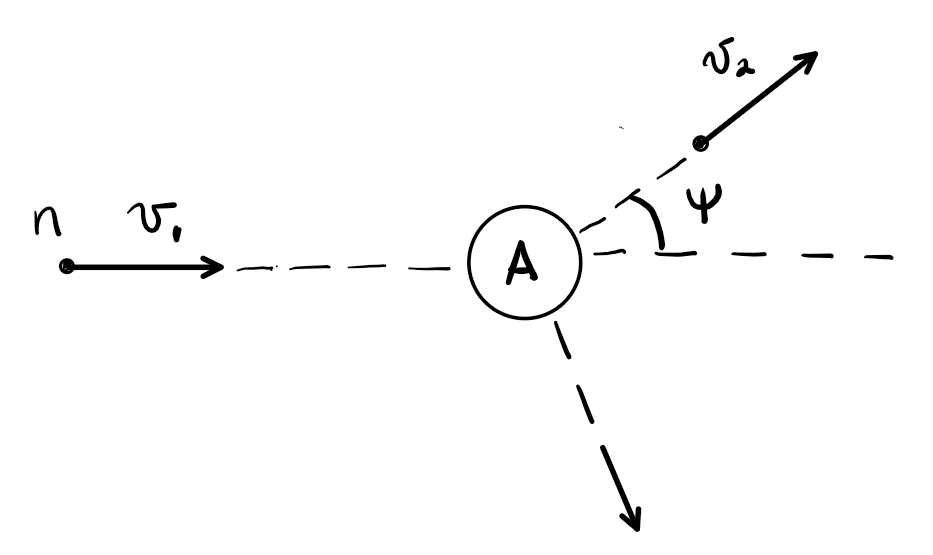
\includegraphics[width=\textwidth]{./Figures/P1/lab.png} 
	      \caption{Lab frame.} 
	      \label{fig:lab}
    \end{subfigure}
    \begin{subfigure}[t]{0.49\textwidth}
    \captionsetup{justification=centering}
	   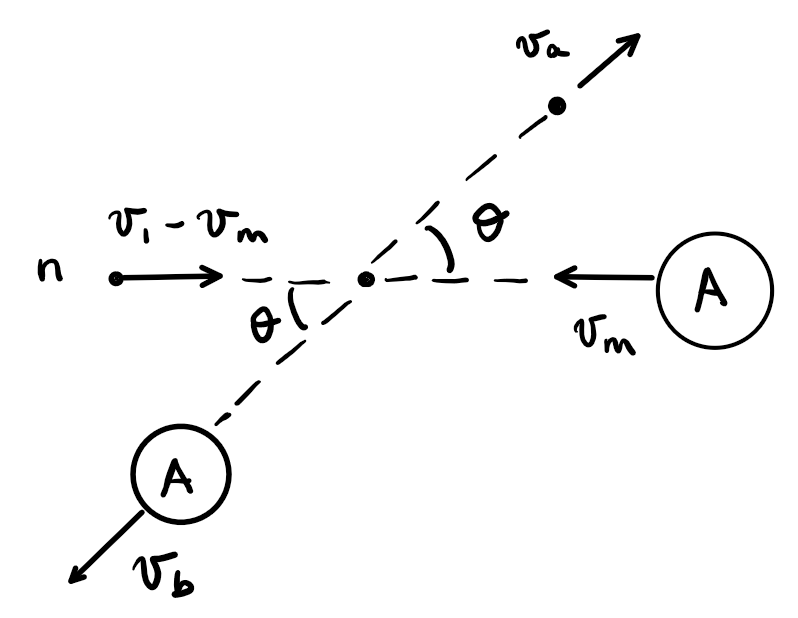
\includegraphics[width=0.75\textwidth]{./Figures/P1/com.png} 
	   \caption{Centre-of-mass (CoM) frame.} 
	   \label{fig:com}
    \end{subfigure}
    \caption{Co-ordinate systems/reference frames for elastic collisions.}
    \label{fig:elastic}
\end{figure*}

First we consider the `lab frame', i.e., how we would see the kinematics occurring as observers in `the lab', shown in Fig.~\ref{fig:lab}. Here n is the incoming neutron, $v_1$ is its initial velocity, and its mass is $M_\mathrm{n} = 1$. The target has a mass $M_\mathrm{target} = A$. On collision, the neutron will deflect at an angle of $\psi$, travelling at a velocity of $v_2$. The total momentum in this system is:
\begin{equation*}
    \sum_i v_i M_i = v_1 \times 1 + 0 \times A = v_1\;\mathrm{.}
\end{equation*}
The kinetic energy of the system is:
\begin{equation*}
    \mathrm{KE}_\mathrm{Lab} = \frac{1}{2}v^2_\mathrm{1}\;\mathrm{.}
\end{equation*}

The centre of mass of the system will move as the neutron moves towards the target. The centre of mass velocity is given as the weighted sum of the particle velocities:
\begin{equation*}
    v_\mathrm{m} = \frac{v_1M_\mathrm{n} + 0\times M_\mathrm{target}}{M_\mathrm{n}+M_\mathrm{target}} = \frac{v_1}{1+A}\;\mathrm{.}
\end{equation*}
From this we can create a simpler reference frame by \textbf{fixing the centre of mass to be stationary} -- this will be referred to as the Centre of Mass (CoM) system. Given that the CoM does not move, other particles must move relative to it (shown in Fig.~\ref{fig:com}). The net neutron velocity before collision then becomes:
\begin{equation*}
    v_1 - v_\mathrm{m} = v_1\left(1 - \frac{1}{A+1}\right) = v_1\frac{A}{A+1}\;\mathrm{,}
\end{equation*}
and its momentum is identically:
\begin{equation*}
    1 \times (v_1 - v_\mathrm{m}) = v_1\frac{A}{A+1}\;\mathrm{.}
\end{equation*}
The target also has a relative velocity, which is simply $-v_\mathrm{m}$ and a momentum of: \begin{equation*}
    -v_\mathrm{m}A = -v_1\frac{A}{1+A}\;\mathrm{.}
\end{equation*}
Hence the total momentum of the system is zero. The kinetic energy of the system is:
\begin{equation*}
    \mathrm{KE}_\mathrm{CoM} = \frac{1}{2}\left(v_1 - v_\mathrm{m}\right)^2 + \frac{1}{2}Av^2_\mathrm{m} = \frac{1}{2}v^2_1\frac{A}{A+1}\;\mathrm{.}
\end{equation*}

%This allows us to relate the kinetic energies between the two systems:
%\begin{equation*}
%    \mathrm{KE}_\mathrm{CoM} = \frac{A}{A+1}\mathrm{KE}_\mathrm{Lab}\;\mathrm{.}
%\end{equation*}
We must conserve both energy and momentum in the collision. This will allow us to relate the outgoing velocities to the incoming velocities. Our KE balance is:
\begin{equation*}
    \frac{1}{2}v^2_1\frac{A}{A+1} = \frac{1}{2}v^2_\mathrm{a} + \frac{1}{2}Av^2_\mathrm{b}\;\mathrm{.}
\end{equation*}
Given that the total momentum is zero, the momentum balance reduces to:
\begin{equation*}
    v_\mathrm{a} = v_\mathrm{b}A\;\mathrm{.}
\end{equation*}
Solving for the outgoing velocities we get:
\begin{equation*}
    v_\mathrm{a} = \frac{A v_1}{A+1}\;\mathrm{,}
\end{equation*}
\begin{equation*}
    v_\mathrm{b} = \frac{v_1}{A+1}\;\mathrm{.}
\end{equation*}

But now we need to get back to the lab system in order to work out the neutron energy loss. The two systems move relative to each other with a velocity $v_\mathrm{m}$ such that:
\begin{equation*}
    \vec{v}_2 = \vec{v}_\mathrm{a} + \vec{v}_\mathrm{m}\;\mathrm{.}
\end{equation*}
This is illustrated in the diagram in Fig.~\ref{fig:system_transform}. 
\begin{figure}[h]
  \centering
  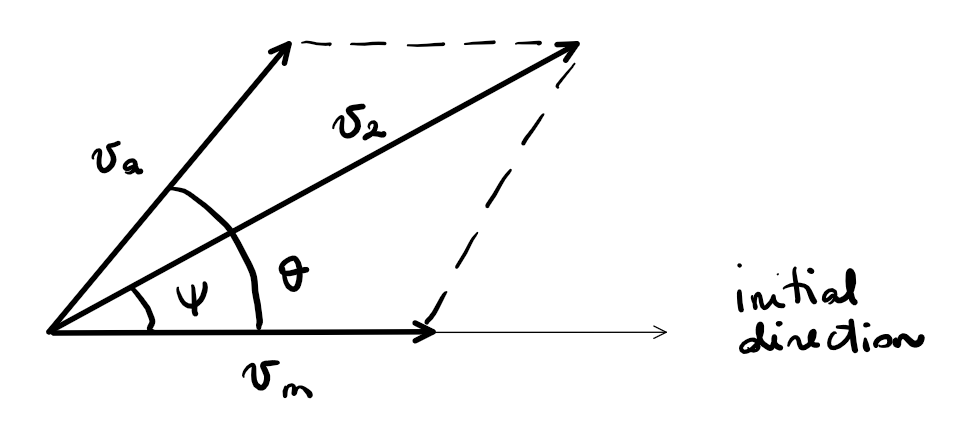
\includegraphics[scale=0.60]{./Figures/P1/outgoing.png} 
  \caption{Geometry of the outgoing collision system.} 
  \label{fig:system_transform}
\end{figure}

Given the geometry of the problem (or vector addition or the law of cosines where $c^2 = a^2 + b^2 + 2ab\cos\theta$), we can relate the magnitudes of the incoming and outgoing velocities as:
\begin{equation*}
    v^2_2 = v^2_1 \frac{A^2 + 2A\cos\theta + 1}{(A+1)^2}
\end{equation*}
We can rewrite the speed relation in terms of the ratio of energies by dividing by $v^2_1$:\begin{equation*}
    \frac{v^2_2}{v^2_1} = \frac{E_2}{E_1} = \frac{A^2 + 2A\cos\theta + 1}{(A+1)^2}\;\mathrm{.}
\end{equation*}
It is common to define a new variable here:
\begin{equation*}
    \alpha \equiv \left(\frac{A-1}{A+1}\right)^2\;\mathrm{,}
\end{equation*}
where $\alpha(\mathrm{hydrogen}) = 0$ and $\alpha(M_\mathrm{target}\rightarrow\infty) = 1$. This lets us rewrite the energy ratio as:
\begin{equation}\label{eq:slowdown}
    \frac{E_2}{E_1} = \frac{(1 + \alpha) + (1-\alpha)\cos\theta}{2}
\end{equation}
This tells us that our minimum energy loss (or maximum $E_2/E_1$) must occur when $\theta = 0$ or $\cos\theta = 1$:
\begin{equation*}
    \max \frac{E_2}{E_1} = \frac{(1+\alpha) + (1-\alpha)}{2} = 1\;\mathrm{.}
\end{equation*}
Conversely, our maximum energy loss occurs if $\theta = \pi$ (a head-on collision and 180$^\mathrm{o}$ deflection):
\begin{equation*}
    \min \frac{E_2}{E_1} = \frac{(1+\alpha) - (1-\alpha)}{2} = \frac{2\alpha}{2} = \alpha\;\mathrm{.}
\end{equation*}
If our target were hydrogen, $\alpha = 0$, i.e., all energy can be lost in a direct collision.

From the same trigonometry as before, we can obtain the cosine of $\psi$:
\begin{equation*}
    \cos\psi = \frac{A\cos\theta + 1}{\sqrt{A^2 + 1 + 2A\cos\theta}}\;\mathrm{.}
\end{equation*}
This implies that:
\begin{equation*}
    \lim_{A\rightarrow\infty} \cos\psi = \cos\theta\;\mathrm{,}
\end{equation*}
i.e., (elastic) scattering becomes more isotropic for heavier nuclei.

Note that an angular element over the unit sphere is given as $\mathrm{d}\Omega = \sin\theta\mathrm{d}\theta\mathrm{d}\varphi$, where $\theta$ is a polar angle and $\varphi$ is an azimuthal angle. This would be integrated from $\varphi = 0, 2\pi$ and $\theta = 0,\pi$ to give the surface area of the unit sphere, $4\pi$ radians. If we assert (from observing physics) that outgoing collision directions tend to depend only on the cosine between the incoming and outgoing direction, we can define the collision angular co-ordinate system such that the cosine is over $\theta$ and therefore scattering is independent of the azimuthal angle (or equi-probable). This reduces our angular element to $\mathrm{d}\Omega = 2\pi\sin\theta \mathrm{d}\theta$. This is visualised in Fig.~\ref{fig:angular}.

\begin{figure}[h]
  \centering
  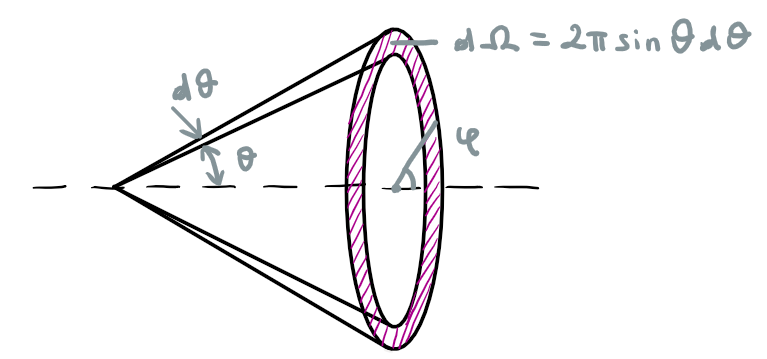
\includegraphics[scale=0.50]{./Figures/P1/angular.png} 
  \caption{Differential angular element for the scattering system with azimuthal symmetry.} 
  \label{fig:angular}
\end{figure}

Given the definition of the differential angular element and s-wave isotropy, the average scattering cosine in the CoM system is 0. For the lab system, this is:
\begin{equation*}
    \overline{\cos\psi} = \frac{\int^\pi_0\mathrm{d}\theta\;\sin\theta\cos\psi}{\int^\pi_0\mathrm{d}\theta\sin\theta} =  \frac{2}{3A}\;\mathrm{.}
\end{equation*}
Once again we can see that $\lim_{A\rightarrow\infty}\overline{\cos\psi}=0$.

Now we can calculate probabilities of scattering from one angle and energy to another angle and energy. Due to isotropy in CoM for s-wave scattering, the probability of scattering  to an angle $\mathrm{d}\theta$ about $\theta$ is simply:
\begin{equation*}
    P(\theta)\mathrm{d}\theta = \frac{\mathrm{d}\Omega}{4\pi} = \frac{2\pi\sin\theta\mathrm{d}\theta}{4\pi} = \frac{1}{2}\sin\theta\mathrm{d}\theta\;\mathrm{.}
\end{equation*}
From Eq.~\eqref{eq:slowdown}, we also know that $\theta$ maps directly to a value of $E_2$, i.e., $E_2 = f(\theta)$, and so we can construct a relationship between the probability density functions (PDFs) of $\theta$ and $E_2$. This relationship will be of the form (given that probability in a differential area must be the same under a change of variables):
\begin{equation*}
   |P(E_2)\mathrm{d}E_2| = | P(\theta)\mathrm{d}\theta|\;\mathrm{.}
\end{equation*}
As standard PDFs must be everywhere positive, this implies that:
\begin{equation}\label{eq:prob_equivalence}
    P(E_2) = P(\theta)\left|\frac{\mathrm{d}\theta}{\mathrm{d}E_2}\right|\;\mathrm{.}
\end{equation}

If we differentiate Eq.~\eqref{eq:slowdown} with respect to $\theta$ we get:
\begin{equation*}
    \mathrm{d}E_2 = \frac{1-\alpha}{2}E_1\;\mathrm{d}\left(\cos\theta\right) = -\frac{1-\alpha}{2}E_1\sin\theta\mathrm{d}\theta\;\mathrm{,}
\end{equation*}
giving:
\begin{equation*}
    \frac{\mathrm{d}\theta}{\mathrm{d}E_2} = -\frac{2}{(1-\alpha)E_1\sin\theta}\;\mathrm{.}
\end{equation*}
Inserting this relationship into Eq.~\eqref{eq:prob_equivalence} gives:
\begin{equation}\label{eq:pdf}
    P(E_2) = \frac{1}{2}\sin\theta\times \frac{2}{(1-\alpha)E_1\sin\theta} = \frac{1}{(1-\alpha)E_1}\;\mathrm{.}
\end{equation}
With this, we can finalise the construction of a PDF for our outgoing energy. The resulting outgoing energy must be between $E_1$ and $\alpha E_1$ (from Eq.~\eqref{eq:slowdown}) and the probability of a given energy is uniform over this range (from Eq.~\eqref{eq:pdf}, there is no dependence on the outgoing energy). Hence, our probability of scattering from $E_1$ to some $E_2$ is:
\begin{equation*}
    P(E_1\rightarrow E_2)\mathrm{d}E_2 = \left\{\begin{array}{ll}
      \frac{\mathrm{d}E_2}{E_1 (1-\alpha)}\;\mathrm{;}\;\; E_2\in [\alpha E_1, E_1]\\
      0\;\mathrm{;}\;\;\mathrm{ otherwise}
      \end{array} 
      \right.
   \;\mathrm{.}
\end{equation*} 
This is illustrated in Fig.~\ref{fig:pdf}. This is an extremely useful result. Note, that this is only true for elastic scattering in light nuclei and for heavier nuclei there will tend to be other angular dependencies from other scattering channels creeping in. In LWRs, however, water is dominant in the physics and this distribution describes the interaction of neutrons and hydrogen very well.

Finally, we can calculate our average energy loss per collision as:
\begin{equation*}
    \overline{\Delta E} = E_1 - \overline{E_2} = E_1 - \int^{E_1}_{\alpha E_1}\frac{E_2\mathrm{d}E_2}{E_1(1-\alpha)} = \frac{1-\alpha}{2}E_1\;\mathrm{.}
\end{equation*}
On average, neutrons will lose half their energy on collision with hydrogen.

\begin{figure}[h]
  \centering
  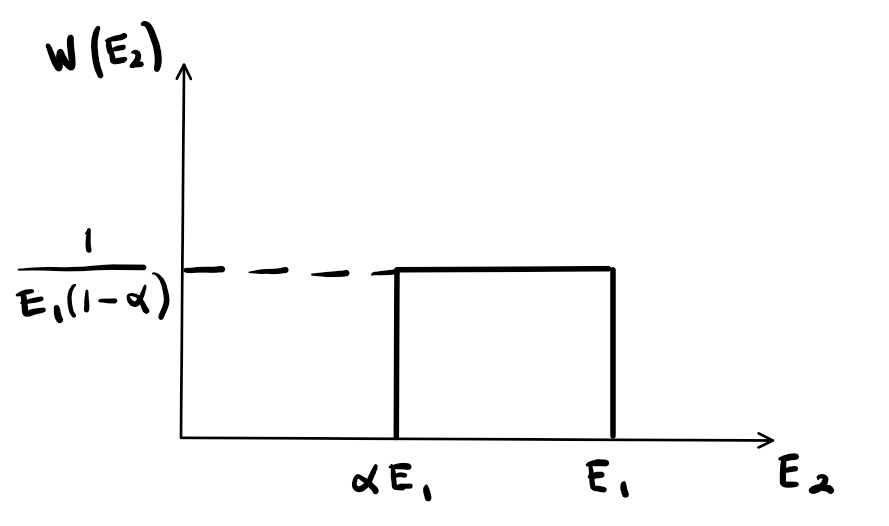
\includegraphics[scale=0.50]{./Figures/P1/probOut.png} 
  \caption{Probability density function for the outgoing neutron energy from elastic collisions.} 
  \label{fig:pdf}
\end{figure}

\subsection{Lethargy}

We do not have to work explicitly in terms of neutron energy -- other quantities can be useful in doing the maths too. Often we use the neutron lethargy, defined as:
\begin{equation*}
    u = \ln{\frac{E_0}{E}}\;\mathrm{,}
\end{equation*}
where $u$ is lethargy, $E$ is the corresponding neutron energy, and $E_0$ is some reference neutron energy which should be larger than $E$. Rather than speaking in terms of energy loss per collision, we can speak in terms of lethargy gain per collision. To do this, we need to relate changes in energy to changes in lethargy, the same as we did for angles. This would give:
\begin{equation*}
    |P(u_1\rightarrow u_2)\mathrm{d}u_2| = |P(E_1\rightarrow E_2) \mathrm{d}E_2|\;\mathrm{,}
\end{equation*}
or
\begin{equation*}
    P(u_1\rightarrow u_2) =  P(E_1\rightarrow E_2)\left|\frac{\mathrm{d}E_2}{\mathrm{d}u_2} \right|\;\mathrm{.}
\end{equation*}
Given the definition of lethargy, this is very easy to construct:
\begin{equation*}
    u = \ln{\frac{E_0}{E}}\rightarrow E = E_0 e^{-u}\;\mathrm{,}
\end{equation*}
and so
\begin{equation*}
    \mathrm{d}u = -\frac{\mathrm{d}E}{E} \rightarrow \mathrm{d}E = -E\;\mathrm{d}u\;\mathrm{.}
\end{equation*}
Hence our probability density function is:
\begin{equation*}
    P(u_1\rightarrow u_2) = E_2 P(E_1\rightarrow E_2) = \frac{E_2}{E_1(1-\alpha)}\;\mathrm{,}
\end{equation*}
or
\begin{equation*}
    P(u_1\rightarrow u_2)\mathrm{d}u_2 = \left\{\begin{array}{ll}
      \frac{e^{u_1-u_2} }{1-\alpha}\mathrm{d}u_2\;\mathrm{;}\;\; u_2\in [u_1, u_1 + \ln{(1/\alpha)}]\\
      0\;\mathrm{;}\;\;\mathrm{ otherwise}
      \end{array} 
      \right.
   \;\mathrm{.}
\end{equation*}
Here $\ln (1/\alpha)$ is the maximum lethargy a particle can gain in a collision. Arguably, this may appear to just complicate things, but the value of lethargy becomes more apparent when we start having to integrate many things in energy which look like $\mathrm{d}E/E = -\mathrm{d}u$.

One important lethargy quantity which we will see is the average lethargy gain per collision. This is defined as:
\begin{equation*}
    \xi =\int^{E'}_{\alpha E'}\mathrm{d}E \ln\left(\frac{E'}{E}\right)P(E'\rightarrow E) = 1 + \frac{\alpha}{1-\alpha}\ln\alpha\;\mathrm{.}
\end{equation*}
Note, lethargy becomes a bit more painful to work with when dealing with hydrogen and $\alpha=0$.





